\chapter{New Machine Tutorial}
\label{sec:new_machine_tutorial}
\minitoc

\section{Introduction}

Many research groups from both the machine learning and the neuroscience communities are actively involved in the implementation of new methods for analyzing neuroscience data. In an effort to promote science and the collaboration between researchers across the world, the developers of PRoNTo, while having it as an open-source software right from the start, have also been constantly trying to make it more user-friendly and easy to use. To that end, the whole structure of PRoNTo has been built in such a way, that it makes it relatively easy for a developer or an experienced user to interfere in all steps of the process and customize them to their needs. However, while the customization of all the other steps of the process is much more straight-forward, importing a new method (or `machine', as they are called in PRoNTo), or a wrapper for a library, is a bit more intricate.
\\

This tutorial is intended as a semi-standalone tutorial with the purpose of walking a developer through all the steps required to import their own method into PRoNTo both in Batch and GUI. It will provide all the details on how your machine in your script needs to be structured, as well as the modifications required in all the scripts of PRoNTo to fully port a new method in it and we expect that users with programming experience should be able to use nothing more than this tutorial to import a new method. We will follow closely Chapter \ref{data_example2}, which uses the IXI dataset, therefore even though not necessary, the readers are advised to go through that tutorial first. The IXI dataset can be found on PRoNTo's website \url{http://www.mlnl.cs.ucl.ac.uk/pronto/prtdata.html} (data set \#3). The machine we will use as a toy is the Kernel Ridge Regression (\textit{prt\_machine\_krr}), so some parts (like the arguments passed) will resemble the ones in the \textit{prt\_machine\_krr} script. You will also need to download a compressed copy of the \textit{new\_machine} folder, found in \url{http://www.mlnl.cs.ucl.ac.uk/pronto/new\_machine}, unzip it and put the whole folder (\textit{new\_machine}) inside the \textit{PRoNTo/machines} folder. The \textit{new\_machine} folder includes all the files needed for you to run this tutorial. Inside it you will find:

\bi
\item A file named `prt\_new\_machine.m', which will be the new method tested.
\item A \textit{d} structure example, which is a structure containing all the information of the data that the `prt\_new\_machine.m' accepts as input.
\item And \textit{new\_machine\_batch.mat}, which is a .mat file containing all PRoNTo Batch modules to test your new machine in case you only want to focus on testing your method.
\ei

\noindent \textbf{Note:} Importing a new machine is far more straight-forward through the Batch System, compared to GUI, so users familiar with it are strongly advised to first try their machines in Batch, and only go through the process of porting it in GUI if they intend to use GUI for their analyses.
\\

\noindent \textbf{Note:} Any reference to specific lines in the scripts follow PRoNTo v3.0, so the reader is advised to download that version in order to help themselves find the parts of the code that need to be modified.
\\

PRoNTo is \matlab-based and includes six main modules: `Data \& Design', `Prepare feature set', `Model: Specify new', `Model: Specify from', `Model: Run' and `Compute weights'. For a specific model PRoNTo can display results in terms of performance as well as  the model's weights. Additional review options enable the user to review information about the data, features and models. All modules were implemented using a graphical user interface (GUI) and the \matlab{} SPM Batch System. Using the \matlab{}  Batch System the user can run each module as batch jobs, and you can also extract the jobs you created in .mat files and run them using only scripts, which enables a very efficient analysis framework. Hence, people primarily interested in testing their method, should only focus on section \ref{sec:new_machine_batch} which uses the Batch.
\\

All information about the data, experimental design, models and results are saved in a structure called PRT inside a .mat file called `PRT.mat'. The PRT.mat is first created when you run the `Data \& Design' module. PRoNTo also creates additional files, or overwrites existing ones, during each step (module) of the analysis. Each step of the analysis also updates the PRT.mat itself accordingly. 
\\
% Further details about the Batch System will be provided in the following sections.


In the following section we are first going to explain how to create your own `machine' script according to PRoNTo's standards, together with the structure of the input data, as well as the structure that the output data have to have. In Section \ref{sec:new_machine_batch} we will briefly explain the Batch system, and how to import and run your new machine with it. And finally in Section \ref{sec:new_machine_gui} we will explain how to import your new machine in PRoNTo's GUI.

\section{prt\_new\_machine.m}

First of all the user has to create their own machine script. Once they have created it according to the specifications of PRoNTo, they have to put it inside the \textit{PRoNTo/machines} folder. A template script named `prt\_new\_machine' should already exists inside the folder \textit{PRoNTo/machines/new\_machine}, so the user is advised to use this as a template. Two things are important here. The way the input is structured, so that the user knows how to modify their method to accept the data as they enter their script, as well as the way the user has to structure the output of their script so that it is compatible with the rest of the PRoNTo structures.
\\

\noindent \textbf{\underline{Important note}:} \textbf{The full path of the custom machine must be manually added to the \matlab{} Path.}


\subsection{Inputs}

There are two input structures to the machine function that contain all the relevant information of the data, \textit{d} and \textit{args}.

\begin{enumerate}

\item \textbf{d:} This is the structure containing all the information of the data. The \textit{d} structure contains more fields than what are needed. The most important ones are the following:

\bi

\item \textbf{.tr\_targets:}
training labels (for classification) or values (for regression). This is a column vector of [Ntr x 1] dimensions, where Ntr is the number of targets of the training data.

\item \textbf{.te\_targets:}
testing labels (for classification) or values (for regression). This is a column vector of [Nte x 1] dimensions, where Nte is the number of targets of the testing data.

% \item \textbf{.tr\_id:}

% \item \textbf{.te\_id:}

\item \textbf{.use\_kernel:} Whether the data are in form of kernel matrices (true) or in form of features (false).

\item \textbf{.pred\_type:} Prediction type, `Classification' or `Regression'.

% \item \textbf{.tr\_param:}

% \item \textbf{.te\_param:}

\item \textbf{.train:} Training data (cell array of matrices of row vectors, each having [Ntr x D] dimensions if we input the raw data, or [Ntr x Ntr] if we input their kernels]). Each matrix contains one representation of the data. This is useful for approaches such as multiple kernel learning. % XXXX

\item \textbf{.test:} Testing data (cell array of matrices row vectors, each having [Nte x D] dimensions if we input the raw data, or [Nte x Nte] if we input their kernels]). % XXXX Isn't that the .testcov though?? Can't we input the .train in traincov? or not?!? XXXX

\item \textbf{.testcov:} Testing covariance (cell array of matrices row vectors, each [Nte x Nte]).

\ei

Irrespective of the original type of the data (NIfTI, MEEG or .mat), the data are extracted and/or converted to the \textit{d} structure. While in .mat you could visualize your data right from the start, in the cases of NIfti and MEEG there is no PRoNTo function that lets you visualize your data. A test \textit{d} structure is provided inside the \textit{PRoNTo/machines/new\_machine} folder to help the readers visualize better how the input structure is.

\item \textbf{args:} These are arguments required by each machine. These arguments can be strings, alphanumeric, or numeric characters, they are usually specific to the machine and they are mostly defined as defaults elsewhere.

\end{enumerate}

\subsection{Outputs}
\label{ssecc:outputs}

In order for a new machine to be fully compatible with PRoNTo the outputs of the machine have to be structured in a specific way. The outputs of the machine are all gathered under one structure, named \textit{output}, which has the following fields:

\bi
\item \textbf{.predictions:} Predictions of classification or regression [Nte x D]. This field is mandatory.

\item \textbf{.func\_val:} Values of the decision function [Nte x D]. This field is not always mandatory, but the reader is advised to always have it on their output.
\ei

All the other outputs are optional in most cases. The user is advised to go through the different existing machines, in order to get an idea of how they are structured.
\\

\noindent \textbf{Important note regarding weights:} Depending on your machine, in order for it to be able to visualize the contribution (weights) of different regions/features, some extra outputs might be mandatory. For example, while in kernel machines the weights are computed directly, for non-kernel machines they need to be explicitly computed. Hence, if you want to create a non-kernel machine, it is mandatory for either the coefficients to be in the output structure in order to be computed by PRoNTo, or to compute the weights internally and contain them in the output. A thorough look at the existing machines will give the user a good sense of what is needed when.


\section{How to import and test your new machine in Batch}
\label{sec:new_machine_batch}

In the introduction of this chapter it was mentioned that importing a new machine in Batch is more straight-forward when done through Batch, compared to the GUI. That is because the PRoNTo code regarding the Batch system is already prepared to accept a new custom machine, which is done when defining a model in the `Model: Specify new' and `Model: Specify from' modules so there are absolutely no code modifications required. We assume, however, that the reader is already familiar with the PRoNTo Batch from the previous sections, and if not enough, we strongly advise the reader to go through some tutorials first. More specifically, prior to try importing this new machine with Batch, even though not necessary, it will strongly help the readers if they have first completed the tutorial of Chapter \ref{data_example2}, since we are going to use the same PRT.mat (which is the main structure format file of PRoNTo and everything is done and stored in there) and the same feature set to run the new machine. Finally we remind the reader that the toy machine (KRR) of this tutorial, \textit{prt\_new\_machine.m}, is nothing more than a copy of the \textit{prt\_machine\_krr.m}, used here with a generic name for instructional purposes.
\\

We will discuss quite briefly the main parts needed in order for someone not interested in details to directly proceed, with minimal exposure, to import their own machine in PRoNTo. So anyone wanting to get a better understanding should go through the rest of the manual.
\\

To start with, to launch the toolbox GUI, just type {\tt prt} or {\tt pronto} at the \matlab{} prompt and the main GUI figure will pop up, see Fig.~\ref{fig:mainGUI}. From there on simply click on the processing step needed. Most functions of PRoNTo have been integrated into the {\tt matlabbatch} batching system \cite{matlabbatch} (like SPM8) and the batching GUI is launched from the main GUI by clicking on the {\tt Batch} button. Once in the Batch system, click the `Load Batch' button to load the file named `\textit{new\_machine\_test\_batch.mat}' and you will see 5 modules in the Module List.
\\

As you can see in the PRoNTo GUI, each job (one job being for example to specify the details of a model, or to `run' [train\&test] a model) requires you to input all the information every time you want to run this job. This can be tiresome, and prone to errors since after running the job you have no practical way of retrieving fast the information that you just put. So the whole idea behind Batch is to create a principled way to group a lot of jobs together, be able to run them whenever you want, and be able to save them in a .mat file (using the `Save Batch' button) in order to be able to review and revise them whenever you want to. Each module in the list represents one job. The whole module list is run when you click the `Run Batch' button. Now let's proceed by briefly explaining the 5 different modules in the list.
\\

%For practical purposes, a .mat file named `\textit{new\_machine\_test\_batch.mat}' that contains all the batch modules to run the whole tutorial of Chapter \ref{data_example2} with a new custom machine is also available inside the \textit{PRoNTo/machines/new\_machine} folder for the users that want to focus solely on building a new custom machine. You will of course need to change the file and directory paths accordingly. And you will also need to download the IXI dataset, as well as the \textit{new\_machine} folder.
%\\

\noindent \textbf{Note:} All fields of all modules have a help section which can be found at the bottom of the GUI of the Batch system after clicking on the desired field.

\begin{enumerate}
\item \textbf{Data \& Design:} In this module the user imports all the information related to the data, such as, for example, the type of the data, the regression values for regression problems, covariates, and masks, as well as information about the experimental design.

\bi
\item In this module the user has to change the `Directory' field to the directory they desire to run their analysis. It is in this directory where the PRT.mat file will be created. You first have to right-click and `Unselect All' of the previously saved directory.
\item Change the `Files' field to the directory you have stored the 102 subjects of the IXI data set. They should be in the \textit{IXI/Data/aged/Guys} directory. You first have to right-click and `Unselect All' of the previously saved directories of the 102 subjects.
\item Change the `From file' under `Regression targets (subject)' to the appropriate path where the `Age\_old\_Guys.mat' is located. These are the regression target values of the 102 subjects. You first have to right-click and `Unselect All' of the previously saved directory of the `Age\_old\_Guys.mat' file.
\item And finally change the `File' under `Masks' to the appropriate path where the `SPM\_mask\_noeyes.img' is located. Masks are usually used if we want to throw away some irrelevant information prior to the analysis. For example here the fMRI information from the eyes is irrelevant to our analysis, so we use a standard `no\_eyes' mask to throw away the data from the eyes. You first have to right-click and `Unselect All' of the previously saved directory of the `SPM\_mask\_noeyes.img' mask image file.
\ei

\item \textbf{Feature set/Kernel:} In this module the user creates the feature sets from the loaded data in the previous module, in order to be used later on when we build our models. Depending on the type of your data the fields are different, but generally in this module, after defining the data format, you can choose whether to include based on samples or conditions, for example in the case of NIfTI images whether to include all voxels or part of them, some simple extra preprocessing steps, etc.

\bi
\item Here you only need to make sure you have the appropriate directory in the `Load PRT.mat' field.

\noindent \textbf{Note:} When you first create a batch of jobs in the Batch, there is no `PRT.mat' yet created. In that case you can either run the first module by itself, and then click `Specify' to choose the already created PRT.mat, and then run the rest of the modules. Or you can run them all together by using the `Dependency' button. By clicking the `Dependency' button you can choose for example the `Data \& Design' module, which instructs the `Load PRT.mat' field of the `Feature set/Kernel' module to harvest the `PRT.mat' of the `Data \& Design' module to be run as the PRT.mat of this module (`Feature set/Kernel').

\ei

\item \textbf{Model: Specify new:} In this module the user imports all the information related to the machine learning models they want to build, such as whether you want to do classification or regression, which feature sets to use, as well as all the information about the machine learning algorithm itself and the model selection and cross-validation schemes.

\bi
\item First make sure you have the appropriate directory in the `Load PRT.mat' field. Please note the instructions in the previous module about how to use the `Dependency' button.
\item Change the `Function' under the `Custom machine' to the appropriate path where the `prt\_new\_machine.m' is located.
\ei

\item \textbf{Model: Run:} The purpose of this module is pretty simple. Here the user only defines which models they want to run, and whether or not to do permutation test or not.

\bi
\item Here you only have to make sure you have the appropriate directory in the `Load PRT.mat' field.
\ei

\item \textbf{Compute weights:} The previous modules allow the user to specify and run one or more models. These include the machine to be used, the cross-validation scheme and the classifcation/regression problem. The estimation of those models led to predictions on unseen/test data (in each fold), from which measures of performance of the model can be derived
and displayed. In addition, as PRoNTo primarily uses linear models, it provides the option of recovering the model weights in the original feature space, and transforming the weights vector into an image, or map. These maps contain at each feature the corresponding weight of the linear model (that together define the predictive function), and which related to how much this particular feature contributed to the classification/regression task in question. The purpose of this module is to compute those model weights.

\bi
\item Here you only have to make sure you have the appropriate directory in the `Load PRT.mat' field.
\ei

\end{enumerate}

If everything was done properly, clicking the green `Run Batch' button will finish smoothly and give you the same results as the KRR model in Chapter \ref{data_example2}.
\\

At this stage the user should be familiar enough with the Batch in order to do a first test, running the template new machine we provide. It is strongly advisable that the users go in debug mode and enable a breakpoint in the start of the \textit{prt\_new\_machine.m} script to study the two input main input structures (\textit{\textbf{d}} and \textit{\textbf{args}}) directly through the \matlab{} workspace in order to gain a better understanding.
\\

\subsubsection{Create your own Batch from scratch}

The users that want to create the whole batch from scratch by themselves should first follow and finish the regression tutorial of Chapter \ref{data_example2} and, after that, proceed to the additional instructions below.

\bi
\item First open the Batch and fill it in as instructed in \ref{ssec: model_spec_new_krr} but without filling in the `Machine type' field. For practical purposes, change the `Cross-validation type' from `Leave one subject out' to `k-folds CV on subjects' with `k=5'.

The `Model: Specify new' module at this point should look similar to figure \ref{fig:new_machine_tutorial_model_specify_new_custom}.

\begin{figure}[!h]
	\centering
		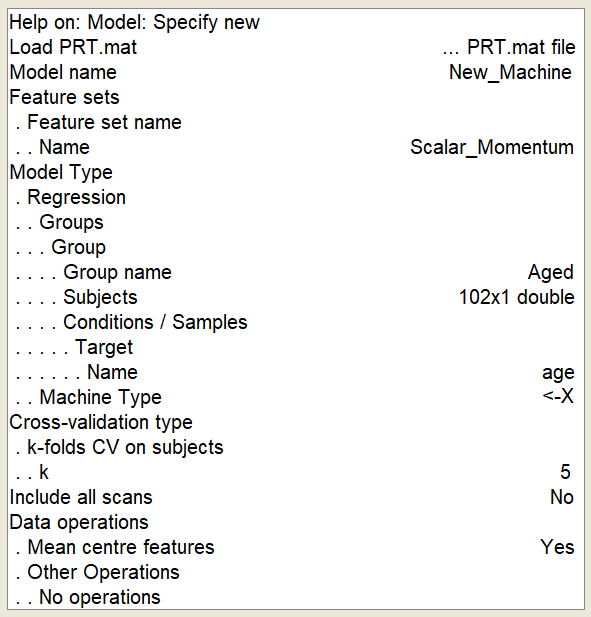
\includegraphics[scale=0.6]{new_machine_tutorial/new_machine_tutorial_model_specify_new_custom.png}
	\caption{`Model: Specify new' module.}
	\label{fig:new_machine_tutorial_model_specify_new_custom}
\end{figure}

\item Now we will describe how to fill the additional field that we skipped before, `Machine type'. Since KRR uses kernels, select the `Kernel machine' option, and, after that, in the `Kernel machine' field, select the `Custom machine' option. There are in total 3 fields here, 2 of which are new.

\begin{enumerate}

\item \textbf{Function:} You need to fill in the full path of your machine's file. In this particular case we have put the machine inside a folder named `new\_machine' so the full path would be something like `PRoNTo/machines/new\_machine/prt\_new\_machine.m'.

\item \textbf{Custom machine string arguments:} These are string parameters specific to each machine. They are usually required if the machine calls an external library for computations. These are the same string parameters mentioned in \ref{sssec:string_params}, so the reader is referred to this subsubsection for a further explanation. In our case, our custom machine requires no string arguments, so leave this field as it is.

\item \textbf{Custom machine optimization and parameters:} This is the same as the `Machine optimization and parameters' of the rest of the machines, with the only exception that no values are auto-filled. First select `Optimize hyper-parameter' and in the `Regularization hyper-parameter' insert the values $[0.01 0.1 1 10 100 1000]$. Finally change the `Cross-validation type for hyper-parameter optimization' to `k-folds CV on subjects' with k=4.

\bi
\item In case you do not want to do a nested cross-validation, you have to select the `No optimization', and in the `No optimization' field you should fill in any default parameter values that your machine requires. In our case that is the value of the $\lambda$ parameter, and is equal to 1. For further information regarding default parameter values the reader is referred to \ref{sssec:def_param_values}.
\ei

\end{enumerate}

\ei

The `Model: Specify new' module finally at this point should look similar to figure \ref{fig:new_machine_tutorial_model_specify_new_custom_final}.

\begin{figure}[!h]
	\centering
		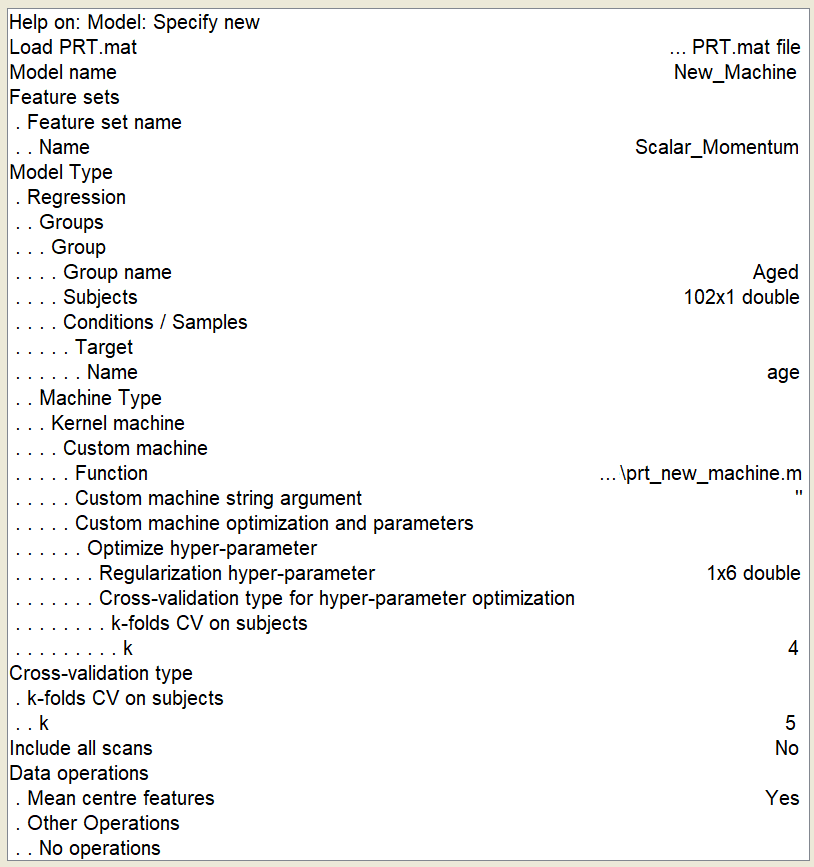
\includegraphics[scale=0.6]{new_machine_tutorial/new_machine_tutorial_model_specify_new_custom_final.png}
	\caption{Final configuration of the `Model: Specify new' module.}
	\label{fig:new_machine_tutorial_model_specify_new_custom_final}
\end{figure}



% \subsection{prt\_get\_machine.m}
% \lstinputlisting[firstline=87,lastline=102, firstnumber=87]{new_machine_tutorial/prt_get_machine.m}




% ===========================================================================


% ===========================================================================




\section{How to import your new machine in GUI}
\label{sec:new_machine_gui}

\subsection{prt\_defaults.m}

This is the script that sets most of the defaults used by PRoNTo. Each machine and/or library has its own parameters that might need to be set as defaults. You have to modify this script to include any default parameters your machine requires. There are 3 things you have to modify in this script.

\subsubsection{Machine lists for GUI}
\label{sssec:machine_lists}

Here we provide the GUI of PRoNTo with a list of names for each machine available. All names can be found inside \textbf{prt\_def.machine}. The names of the machines are grouped according to whether the machine is for classification or regression, whether it uses kernels or not, and whether it is a multi-kernel method or not. In our case since our toy method is KRR (named `New Machine'), which is for regression and uses kernels, we will need to add it to \textit{prt\_def.machine.reg\_K}.

\lstinputlisting[firstline=93,lastline=96, firstnumber=93]{new_machine_tutorial/prt_defaults.m}


\subsubsection{String parameters}
\label{sssec:string_params}

Some times machines require string arguments in their input, especially machine that are wrapper for libraries. Any string arguments your machine might require need to be defined here. Our toy machine (KRR) does not require any string arguments, so for an example we will present the string arguments required to run an L2-SVM as well as an $\epsilon$-SVR using the LIBSVM library.

\lstinputlisting[firstline=105,lastline=109, firstnumber=105]{new_machine_tutorial/prt_defaults.m}

If your machine required some string arguments to work, you would need to define the field \textit{prt\_def.model.new\_machine\_sargs} together with its proper string arguments. You should remember the name you give to this field (.new\_machine\_sargs) because you are going to use it later on.

\subsubsection{Default parameter values}
\label{sssec:def_param_values}

Besides string arguments, some machines may also require numeric values to be set as defaults. For example:

\lstinputlisting[firstline=128,lastline=133, firstnumber=128]{new_machine_tutorial/prt_defaults.m}

In this particular case, the default parameter values required by our toy machine (KRR) are the same as the LIBSVM and LIBLINEAR defaults shown above, so there is no need to add new ones explicitly. We are going to use this when asked in the next subsection. In case you need to specify new ones, you have to put it inside the \textit{prt\_def.model} structure. So your newly defined defaults would need to be inside a structure \textit{prt\_def.model.name\_args} where `name\_args' can be whatever name you want to give to your machine's arguments. You should remember this name because you are going to also use it later on.
\\

\noindent \textbf{Important Note:} The order with which the default parameter values will be harvested is the same as the one that are defined. So the user is advised to pay attention to that order since the machine will most likely not hit an error if run with transposed default parameter values.


\subsection{prt\_get\_machine\_ui.m}

This script is called when you use the GUI, to harvest the defaults you previously defined for each machine\footnote{\textit{prt\_get\_machine.m} is the equivalent of \textit{prt\_get\_machine\_ui.m} but for Batch. Modifications to \textit{prt\_get\_machine.m} will be discussed in the next section.}. You have to modify these scripts to properly harvest your machine’s defaults by including your machine in both of them. Be careful, however, because the GUI and the Batch have small differences in how they define things. Below is an example of how we defined our new machine, which is the same as KRR. First is an example from \textit{prt\_get\_machine\_ui.m}, and then from \textit{prt\_get\_machine.m}.

\lstinputlisting[firstline=110,lastline=122, firstnumber=110]{new_machine_tutorial/prt_get_machine_ui.m}

As we see in the code above, it is in this part that we are asking for the default parameter values that were defined in the previous section. If a new machine required different default parameter values, the user would have defined in the previous section, giving them a specific name, which would have been used in place of \textit{def.libsvmargs} in line \#113.


\subsection{prt\_ui\_copy\_model.m}

This is the script responsible for the GUI of the `Model: Specify from' module. Just as in \ref{sssec:machine_lists}, the user has to put the name of their machine here as well, in two instances, inside the if-loops \#970-1002 and \#1232-1296.

\subsubsection{First instance}

\lstinputlisting[firstline=993,lastline=1002, firstnumber=993]{new_machine_tutorial/prt_ui_copy_model.m}

\subsubsection{Second instance}

\lstinputlisting[firstline=1271,lastline=1291, firstnumber=1271]{new_machine_tutorial/prt_ui_copy_model.m}



\subsection{prt\_plot\_nested\_cv.m}

This script plots the results of the nested cv that appear on \textit{prt\_ui\_results}. The user has to modify the script, by including an extra case in the switch-loop of lines \#27-132, with their machine. Since our toy machine for this tutorial is KRR, we will be using logscale as well, and the x and y labels are also going to be the same.

\lstinputlisting[firstline=66,lastline=79, firstnumber=66]{new_machine_tutorial/prt_plot_nested_cv.m}



\subsection{prt\_weights\_*.m}

As mentioned in \ref{ssecc:outputs} in the note regarding weights, depending on your machine, in order for it to be able to visualize the contribution of different regions/features, some extra outputs might be mandatory. In general, in most cases weights are computed by \textit{prt\_weights\_linkernel.m}. So depending on your machine you might either use one of the existing  scripts, or you might need to create your own new \textit{prt\_weights\_*.m} for building the weights of your new custom machine. That, however, is depended on your machine so the user is advised to go through the existing \textit{prt\_weights\_*.m} scripts to further understand how they might need to structure theirs.


\subsection{Running your new machine}

If your machine's script is properly defined, and if everything was done accordingly, when you open the `Model: Specify new/from' modules, you are going to see your new custom machine as one of the options in the drop-down list like in figure \ref{fig:new_machine_tutorial_gui_model}.

\begin{figure}[!h]
	\centering
		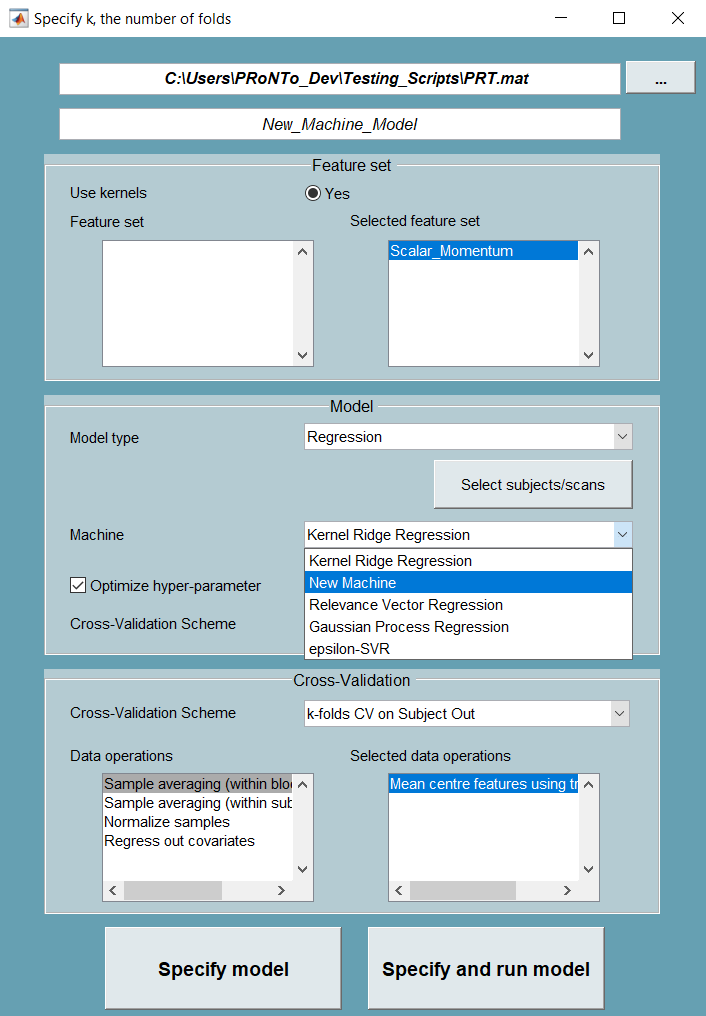
\includegraphics[scale=0.6]{new_machine_tutorial/new_machine_tutorial_gui_model.png}
	\caption{`Model: Specify new' module in GUI with the new machine option}
	\label{fig:new_machine_tutorial_gui_model}
\end{figure}





















	
